\section{Aire d'une figure géométrique} 

% remarque : pour qu'un mot se retrouve dans le lexique : \MotDefinition{asymptote horizontale}{} 

\begin{methode*1}[Évaluer une aire]

\begin{exemple*1}
\begin{minipage}[c]{0.55\textwidth}
 À l'aide du quadrillage, détermine un encadrement de l'aire de la surface jaune, en prenant pour unité un carreau bleu.
 \end{minipage} \hfill%
 \begin{minipage}[c]{0.2\textwidth}
 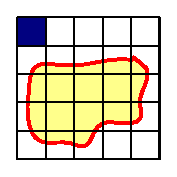
\includegraphics[width=2.3cm]{aire1}
 \end{minipage} \\
 
 \begin{minipage}[c]{0.1\textwidth}
  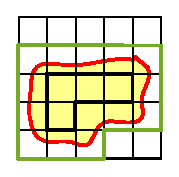
\includegraphics[width=2.3cm]{aire2}
 \end{minipage} \hfill%
 \begin{minipage}[c]{0.7\textwidth}
La surface délimitée en \textbf{\textcolor{H1}{vert}} a une aire plus grande que celle délimitée par la courbe rouge. On compte le nombre de carreaux. Son aire est 18 carreaux.
 \end{minipage} \\[1em]
La surface délimitée en \textbf{noir} a une aire plus petite que celle délimitée par la courbe rouge. On compte le nombre de carreaux. Son aire est quatre carreaux.

Donc l'aire de la figure jaune est comprise entre 4 et 18 carreaux.

\end{exemple*1}

\exercice 
\begin{minipage}[c]{0.50\textwidth}
 Détermine l'aire, en nombre de carrés, des deux figures ci-contre.
 \end{minipage} \hfill%
 \begin{minipage}[c]{0.16\textwidth}
 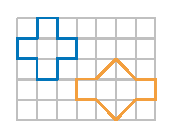
\includegraphics[width=2.2cm]{aire3}
 \end{minipage} \\
%\correction
 
\end{methode*1}

%%%%%%%%%%%%%%%%%%%%%%%%%%%%%%%%%%%%%%%%%%%%%%%%%%%%%%%%

\vspace{2em}


\begin{aconnaitre}[Les longueurs]
Les \MotDefinition{facteurs de multiplication}{} des \textbf{\textcolor{H1}{m (mètres)}} sont :
\begin{colitemize}{2}
\item \textbf{k} (kilo) : $\numprint{1000} = 10^3$ ;
\item \textbf{h} (hecto) : $100 = 10^2$ ;
\item \textbf{da} (déca) : $10 = 10^1$ ;
\item \textbf{d} (déci) : $0,1 = 10^{-1}$ ;
\item \textbf{c} (centi) : $0,01 = 10^{-2}$ ;
\item \textbf{m} (milli) : $0,001 = 10^{-3}$.
\end{colitemize}
\end{aconnaitre}

\vspace{2em}

\begin{methode*1}[Transformer des unités de longueurs]

\begin{exemple*1}
Transforme $0,5$ km en m.

Les m (mètres) sont l'unité de mesure.

$1$ km = $\numprint{1000}$ m, donc $0,5$ km $= 0,5 \cdot \numprint{1000}$ m = $500$ m
\end{exemple*1}

\exercice 
Effectue les conversions d'unités de longueurs suivantes :
\begin{colenumerate}{3}
 \item $50$ cm en m ;
 \item $100$ mm en m ;
 \item $2,3$ hm en m ;
 \item $0,03$ dm en m ;
 \item $23$ dam en cm ;
 \item $4$ cm en hm.
 \end{colenumerate}
%\correction

\end{methode*1}

\newpage

\begin{aconnaitre}[Les aires]
Les \MotDefinition{facteurs de multiplication}{} des \textbf{\textcolor{H1}{m\up{2} (mètres carrés)}} sont :
\begin{colitemize}{2}
\item \textbf{k} (kilo) : $\numprint{1000000}$ ;
\item \textbf{h} (hecto) : $\numprint{10000}$ ;
\item \textbf{da} (déca) : $100$ ;
\item \textbf{d} (déci) : $0,01$ ;
\item \textbf{c} (centi) : $\numprint{0,0001}$ ;
\item \textbf{m} (milli) : $\numprint{0,000001}$.
\end{colitemize}
\end{aconnaitre}

\vspace{4em}

\begin{methode*1}[Transformer des unités d'aires]

\begin{exemple*1}
Transforme $3$ hm\up{2} en m\up{2}.

$1$ hm\up{2} = $\numprint{10000}$ m\up{2}, donc $3$ hm\up{2} $= 3 \cdot \numprint{10000}$ m\up{2} = $\numprint{30000}$ m\up{2}
\end{exemple*1}

\exercice 
Effectue les conversions d'unités d'aires suivantes :
\begin{colenumerate}{3}
 \item $7$ dm\up{2} en m\up{2} ;
 \item $200$ cm\up{2} en m\up{2} ;
 \item $3,2$ hm\up{2} en m\up{2} ;
 \item $0,8$ dm\up{2} en m\up{2} ;
 \item $45$ hm\up{2} en dm\up{2} ;
 \item $400$ cm\up{2} en dam\up{2}.
 \end{colenumerate}
%\correction

 \end{methode*1}




%%%%%%%%%%%%%%%%%%%%%%%%%%%%%%%%%%%%%%%%%%%%%%%%%%%%%%%%

\newpage


\begin{aconnaitre}
\begin{tabularx}{\linewidth}{|c|X|X|}
 \cline{2-3}
\multicolumn{1}{c|}{} & \begin{center} \textbf{\textcolor{H1}{Rectangle}} 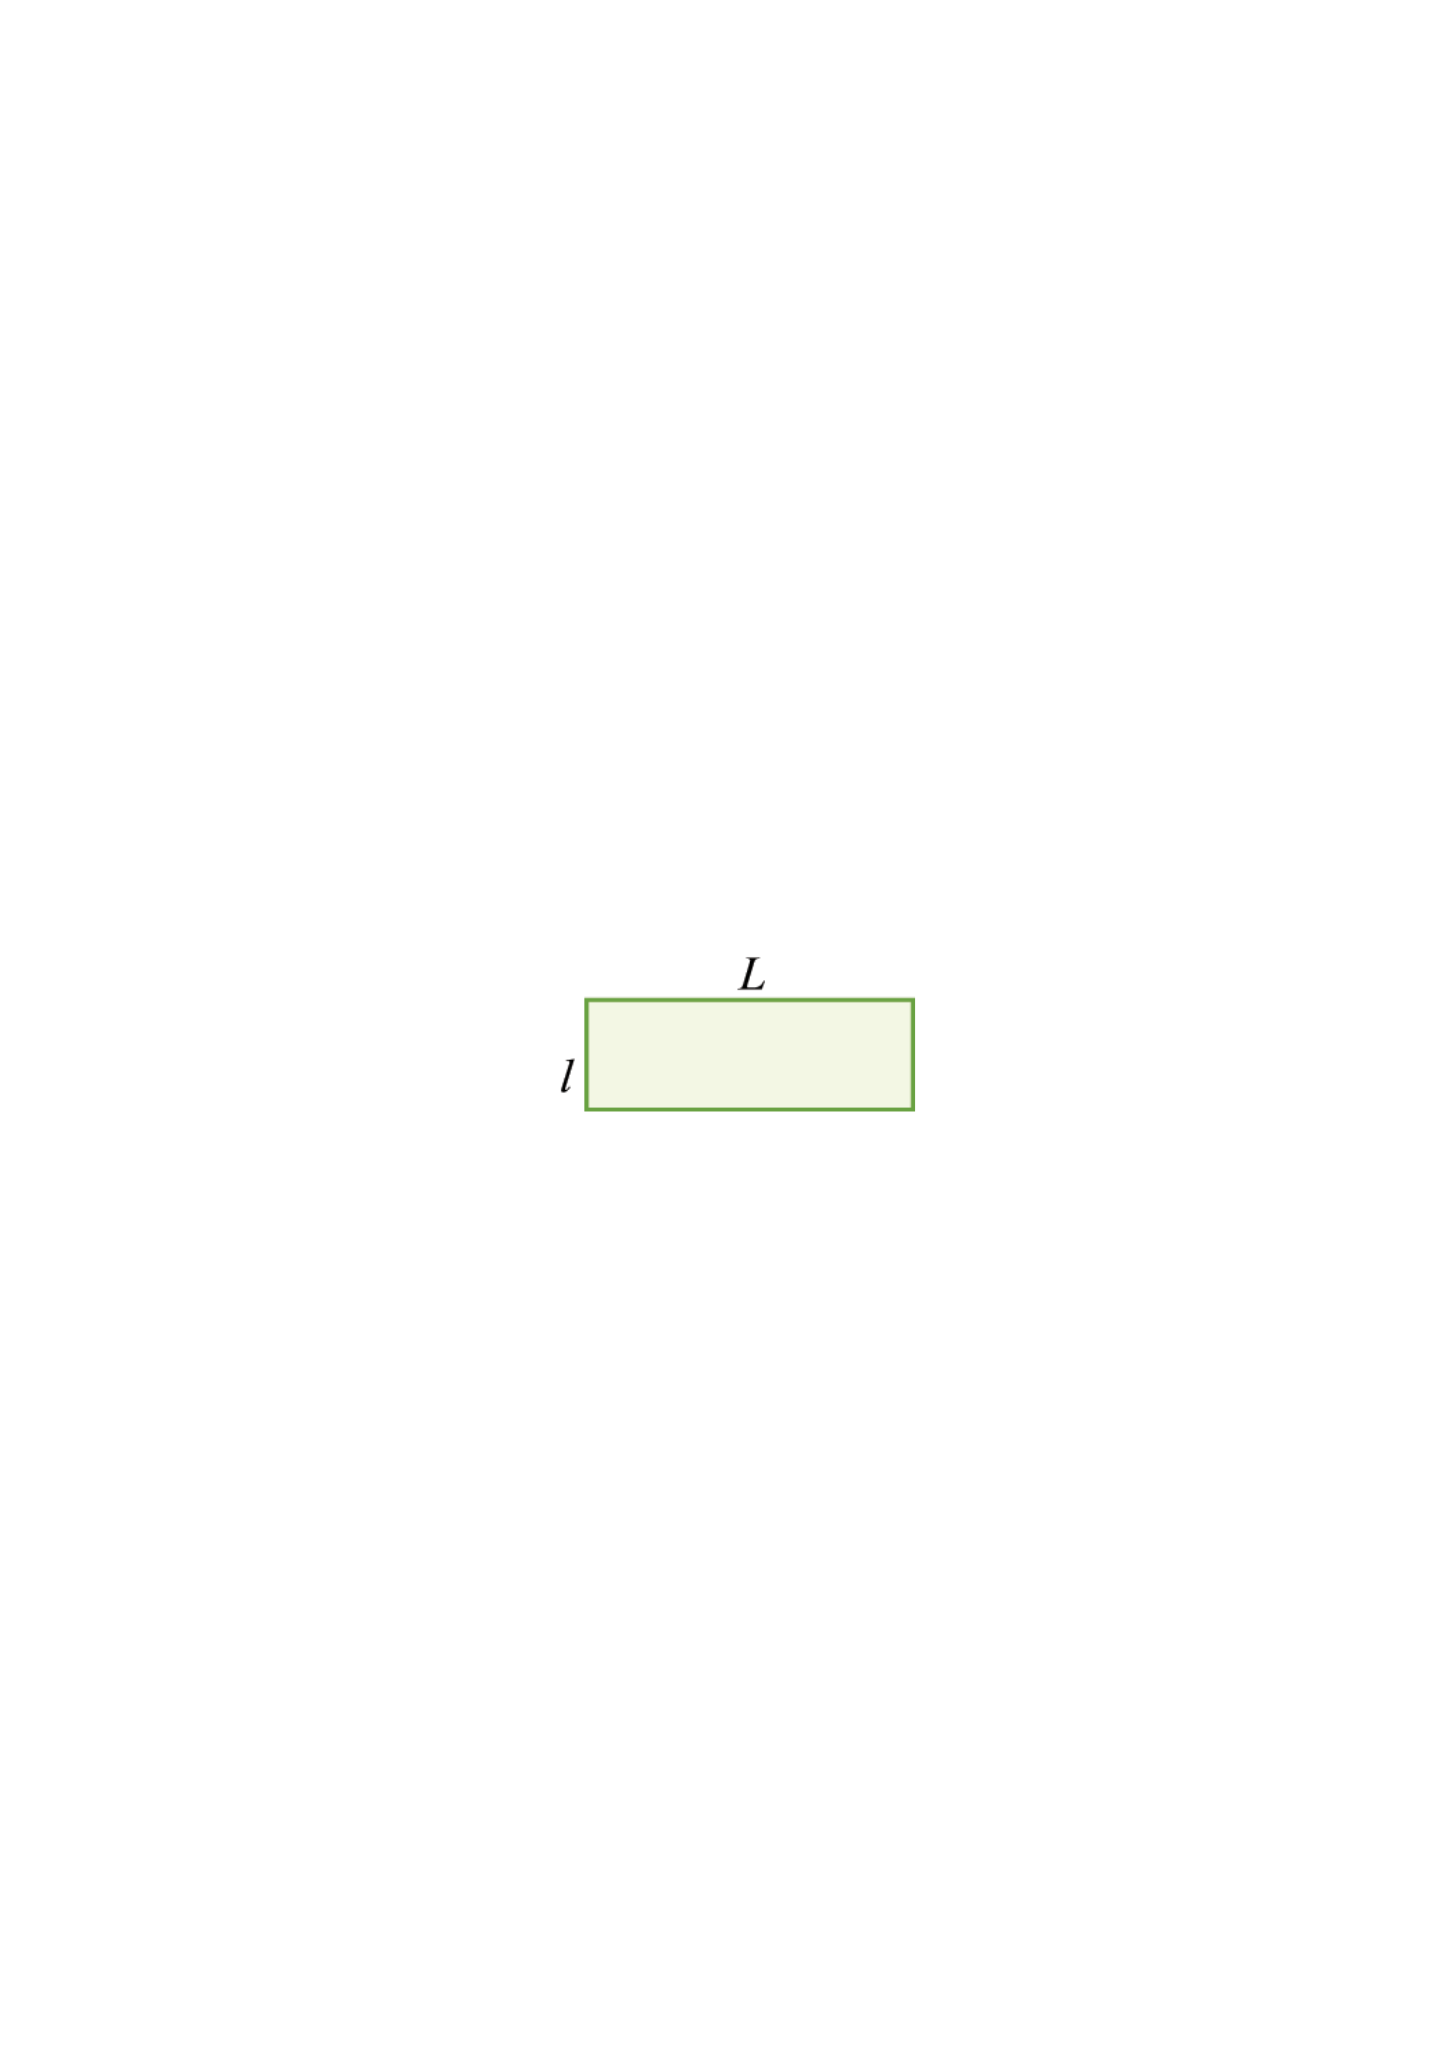
\includegraphics[width=2.5cm]{rectangleLI} \end{center} & \begin{center} \textbf{\textcolor{H1}{Triangle rectangle}} 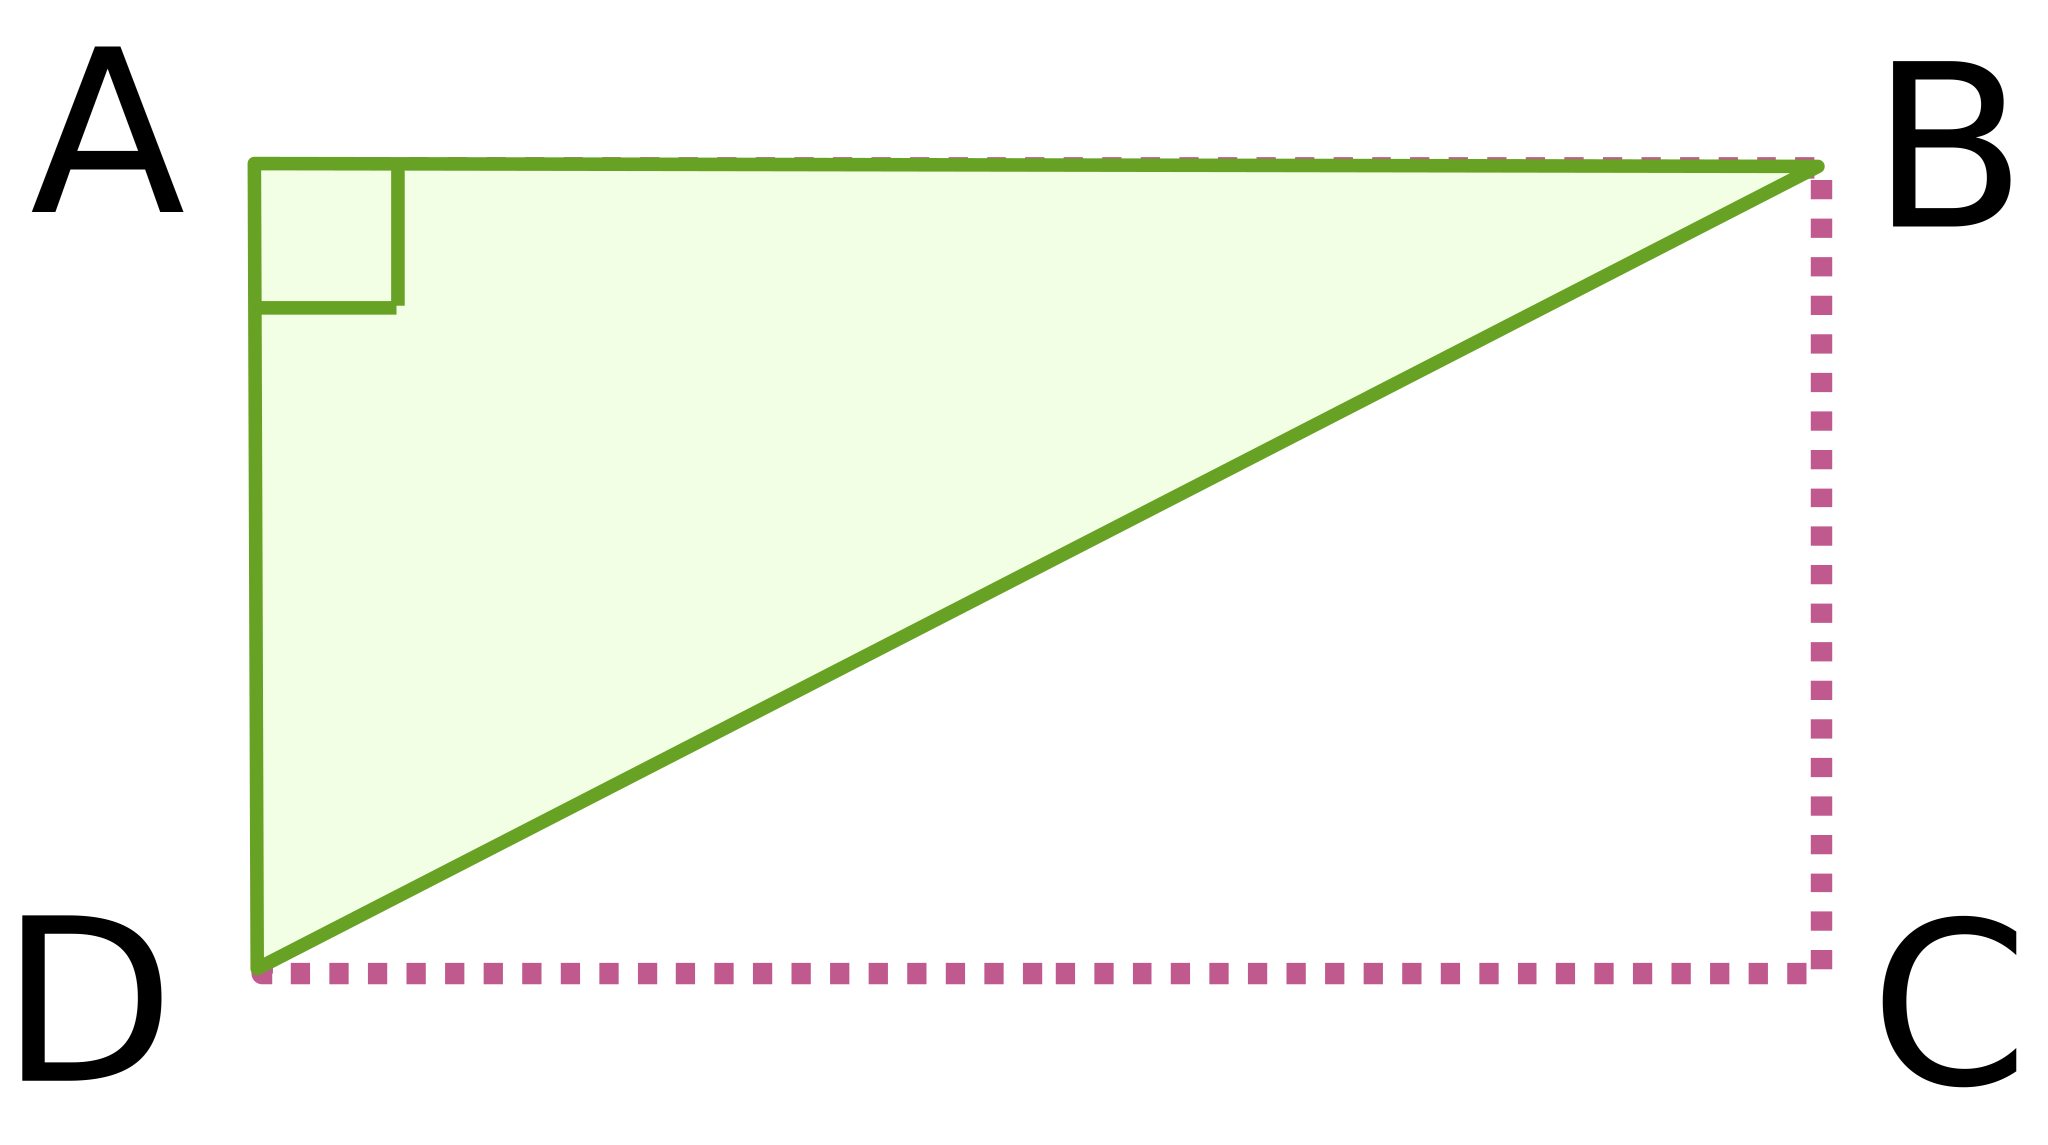
\includegraphics[width=2.7cm]{rectangleABCD4} \end{center} \\ \hline
Formule & L'aire du rectangle peut se calculer avec cette formule : {\large \textbf{$\mathcal{A} = L \cdot \ell$}} & L'aire de $ABD$ est égale à la moitié de l'aire de $ABCD$ : {\large \textbf{$\mathcal{A} = \dfrac{AB \cdot AD}{2}$}} \phantom{retourligne} \\\hline
 \end{tabularx} \\[1em]
Les longueurs doivent être exprimées dans la même unité.
\end{aconnaitre}



\vspace{2em}

\begin{methode*1}[Calculer des aires à l'aide d'une formule]

\begin{exemple*1}
Calcule l'aire de la figure $ABCDE$ ci‑dessous (L'unité de longueur est le centimètre) :
\begin{center}  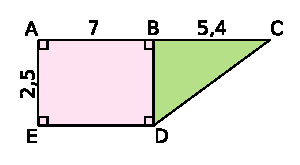
\includegraphics[width=4.3cm]{aire4} \end{center}

 \begin{itemize}
  \item La figure est composée du rectangle $ABDE$ et du triangle rectangle $BCD$. Son aire est donc égale à la somme de l'aire de $ABDE$ et de l'aire de $BCD$ ;
  \item $\mathcal{A}_{ABDE} = AB \cdot AE = 7$ cm $\cdot$ $2,5$ cm = $17,5$ cm\up{2} ; \\[0.2em]
  \item $\mathcal{A}_{BCD} = \dfrac{BC \cdot BD}{2} = \dfrac{5,4 \text{ cm} \cdot 2,5 \text{ cm}}{2} = \dfrac{13,5 \text{ cm}\up{2}}{2} = 6,75 $ cm\up{2} ;\\[0.2em]
  \item $\mathcal{A}_{ABCDE} = 17,5$ cm\up{2} $+ 6,75$ cm\up{2} = $24,25$ cm\up{2}.
  \item L'aire de la figure $ABCDE$ est donc égale à $24,25$ cm\up{2}.
  \end{itemize}
\end{exemple*1}

\exercice 
Détermine l'aire d'un carré de côté 6 cm. 
%\correction

\exercice 
Détermine l'aire d'un rectangle de longueur 3 cm et de largeur 22 mm en donnant le résultat en cm\up{2}.
%\correction
     
\exercice 
$SON$ est un triangle rectangle en $S$, tel que 

$SO = 8,04$ dm et $SN = 0,93$ m. Détermine son aire en donnant le résultat en m\up{2}.
%\correction
 
\end{methode*1}

%%%%%%%%%%%%%%%%%%%%%%%%%%%%%%%%%%%%%%%%%%%%%%%%%%%%%%%%
\newpage

\section{Aire d'un parallélogramme}

\vspace{2em}

\begin{aconnaitre}
Pour calculer l’\MotDefinition{aire d’un parallélogramme}{}, on multiplie la \textbf{\textcolor{H1}{longueur d'un côté}} par la \textbf{\textcolor{C2}{hauteur}} relative à ce côté :

\vspace{1em}

\begin{tabularx}{\textwidth}{XX}
{\large $\mathcal{A} = b \cdot h$} & 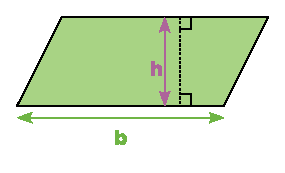
\includegraphics[width=4cm]{parallelogrammehb} \\
 \end{tabularx} \\

\end{aconnaitre}


\vspace{4em}

\begin{methode*1}[Calculer l’aire d’un parallélogramme]


\begin{exemple*1}
Détermine l’\textbf{aire} du parallélogramme suivant :
\begin{minipage}[c]{0.65\textwidth}
\begin{itemize}
 \item On mesure la \textbf{\textcolor{H1}{longueur}} d'un côté ;
 \item On mesure la \textbf{\textcolor{C2}{hauteur}} relative à ce côté ;
 \item On multiplie la longueur du côté repéré par la hauteur relative à ce côté : $\mathcal{A} = 12 \cdot 5 = 60$ ;
 \item L'aire du parallélogramme vaut 60 cm\up{2}.
 \end{itemize}
 \end{minipage} \hfill%
 \begin{minipage}[c]{0.26\textwidth}
 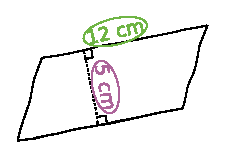
\includegraphics[width=3cm]{parallelog_croquis}
 \end{minipage} \\
\end{exemple*1}

\exercice 
Détermine l’aire des parallélogrammes $MNOP$ et $ABCD$ ci-dessous :
\begin{colenumerate}{2}
 \item 
 
 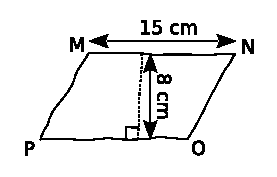
\includegraphics[width=3.7cm]{parallelogMNPO}
 \item 
 
 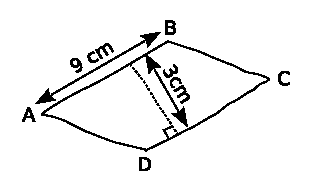
\includegraphics[width=4.4cm]{parallelogABCD}
 \end{colenumerate}
%\correction

\end{methode*1}

%%%%%%%%%%%%%%%%%%%%%%%%%%%%%%%%%%%%%%%%%%%%%%%%%%%%%%%%

\newpage


\section{Aire d'un triangle}

\vspace{2em}

\begin{aconnaitre}
Pour calculer l’aire d’un triangle, on multiplie la \textbf{\textcolor{H1}{longueur d'un côté}} par la \textbf{\textcolor{C2}{hauteur}} relative à ce côté puis on divise le résultat par 2 :

\begin{tabularx}{\textwidth}{XX}
{\large $\mathcal{A} = \dfrac{b \cdot h}{2}$} & 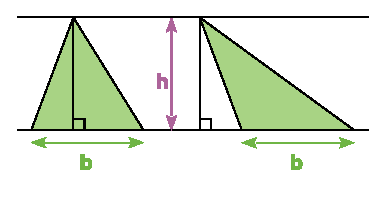
\includegraphics[width=5cm]{longueur_hauteur} \\
 \end{tabularx} \\
 \end{aconnaitre}

\vspace{4em}

\begin{methode*1}[Calculer l’aire d’un triangle]


 
\begin{exemple*1}
Calcule l’aire du triangle suivant :
\begin{minipage}[c]{0.68\textwidth}
\begin{itemize}
 \item On mesure la longueur d'un côté ;
 \item On mesure la hauteur relative à ce côté ;
 \item On multiplie la longueur du côté repéré par la hauteur relative à ce côté puis on divise le résultat par 2 : \\[0.3em]
$\mathcal{A} = \dfrac{10 \cdot 3}{2} = \dfrac{30}{2} = 15$. \\[0.3em]
L'aire du triangle vaut 15 cm\up{2}.
 \end{itemize}
 \end{minipage} \hfill%
 \begin{minipage}[c]{0.2\textwidth}
 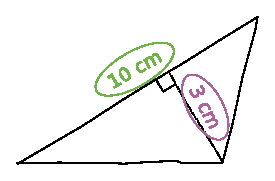
\includegraphics[width=3.5cm]{triangle_croquisZ}
 \end{minipage} \\
\end{exemple*1}


\exercice 
Calcule l’aire des triangles suivants :
\begin{colenumerate}{2}
 \item
 
 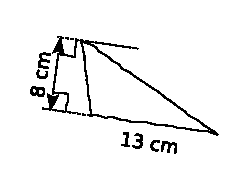
\includegraphics[width=3.1cm]{triangle_croquisY}
 \item
 
 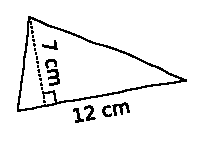
\includegraphics[width=2.8cm]{triangle_croquisW}
 \end{colenumerate}
%\correction

\end{methode*1}

%%%%%%%%%%%%%%%%%%%%%%%%%%%%%%%%%%%%%%%%%%%%%%%%%%%%%%%%

\newpage


\section{Aire d'un losange}

\vspace{2em}

\begin{aconnaitre}
Pour calculer l’aire d’un losange, on effectue le produit des \textbf{\textcolor{H1}{longueurs des diagonales}} puis on divise le résultat par 2 : 

\begin{tabularx}{\textwidth}{XX}
{\large $\mathcal{A} = \dfrac{d \cdot D}{2}$} & 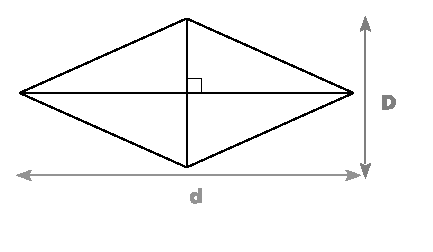
\includegraphics[width=5cm]{losangeDd} \\
 \end{tabularx} \\
 \end{aconnaitre}

\vspace{4em}

\begin{methode*1}[Calculer l’aire d’un losange]


 
 \begin{exemple*1}
Calcule l’aire du losange suivant :
\begin{minipage}[c]{0.68\textwidth}
\begin{itemize}
 \item On repère la longueur des diagonales.
 \item On calcule le produit des longueurs des diagonales puis on divise le résultat par 2 : \\[0.3em]
$\mathcal{A} = \dfrac{10 \cdot 5}{2} = \dfrac{50}{2} = 25$ \\[0.3em]
L'aire du losange vaut 25 cm\up{2}.
 \end{itemize}
 \end{minipage} \hfill%
 \begin{minipage}[c]{0.2\textwidth}
 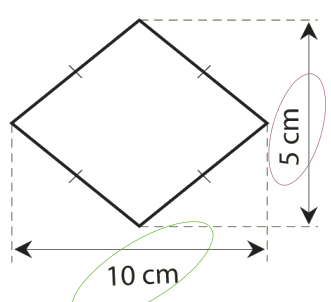
\includegraphics[width=2.9cm]{losange26}
 \end{minipage} \\
\end{exemple*1}

 
 \exercice
Calcule l’aire des losanges suivants :
\begin{colenumerate}{2}
 \item
 
 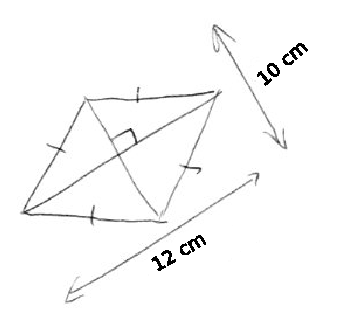
\includegraphics[width=5cm]{losange12_10}
 \item
 
 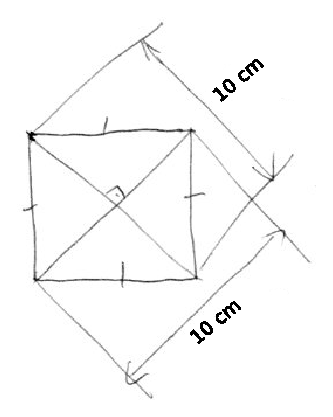
\includegraphics[width=4cm]{losange10_10}
 \end{colenumerate}
%\correction

\end{methode*1}
